\subsection{Разработка лексического анализатора}

% В данном разделе необходимо выполнить разработку алгоритмов функционирования лексического анализатора.

Лексический анализ – процесс разбора входной последовательности символов на распознанные группы – лексемы.

Лексемой является структурная (минимальная значимая) единица языка, состоящая из элементарных символов языка и не содержащая в своём составе других структурных единиц языка \refref{ref:lexlem}.

В ходе выполнения лексического анализатора каждая лексема идентифицируется и преобразуется в токен.

Токен – экземпляр лексемы, представляющий собой пару «тип лексемы» и «значение».
«Тип» указывает на принадлежность лексемы к определенной категории, например, идентификатор, число и т.д.,
а «значение» содержит конкретные данные, соответствующие этой лексеме, оно понадобится на дальнейших этапах.

Категории токенов, которые используются в разрабатываемом предметно-ориентированном языке:
\begin{itemize}
    \item идентификаторы;
    \item числа;
    \item строки;
    \item разделители;
    \item операторы (арифметические, сравнения и т.д);
    \item скобки;
    \item специальные (конец входной последовательности и т.п)
    \item ключевые слова.
\end{itemize}

Полный список токенов с указанием категории и примерами лексем приведен в таблице~\ref{t:tokens}.

Процесс лексического анализа является первым шагов в трансляции исходного кода программы и формирует основу для следующих этапов,
таких как синтаксический анализ и построение абстрактного синтаксического дерева.

\clearpage

\begin{table}[h!]
    \Large
    \centering
    \begin{threeparttable}
        \caption{Токены с примерами}
        \label{t:tokens}
        \begin{tabularx}{\textwidth}{|X|c|c|}
            \hline
            Токен         & Категория      & Пример лексемы  \\
            \hline
            IDENT         & Идентификатор  & qwe             \\
            \hline
            INT           & Число          & 123             \\
            \hline
            STRING        & Строка         & «привет, hello» \\
            \hline
            ASSIGN        & Оператор       & =               \\
            \hline
            PLUS          & Оператор       & +               \\
            \hline
            MINUS         & Оператор       & -               \\
            \hline
            STAR          & Оператор       & *               \\
            \hline
            SLASH         & Оператор       & /               \\
            \hline
            EXCLAMINATION & Оператор       & !               \\
            \hline
            PERCENT       & Оператор       & \%              \\
            \hline
            EQ            & Оператор       & ==              \\
            \hline
            NEQ           & Оператор       & !=              \\
            \hline
            LEQ           & Оператор       & <=              \\
            \hline
            GEQ           & Оператор       & =>              \\
            \hline
            LT            & Оператор       & <               \\
            \hline
            GT            & Оператор       & >               \\
            \hline
            LAND          & Оператор       & \&\&            \\
            \hline
            LOR           & Оператор       & ||              \\
            \hline
            COMMA         & Разделитель    & ,               \\
            \hline
            SEMICOLON     & Разделитель    & ;               \\
            \hline
            LPAR          & Скобка         & (               \\
            \hline
            RPAR          & Скобка         & )               \\
            \hline
            LBRACE        & Скобка         & \{              \\
            \hline
            RBRACE        & Скобка         & \}              \\
            \hline
            LBRACKET      & Скобка         & [               \\
            \hline
            RBRACKET      & Скобка         & ]               \\
            \hline
            IF            & Ключевое слово & if              \\
            \hline
            ELSE          & Ключевое слово & else            \\
            \hline
            TRUE          & Ключевое слово & true            \\
            \hline
            FALSE         & Ключевое слово & false           \\
            \hline
            FUNC          & Ключевое слово & fn              \\
            \hline
            RETURN        & Ключевое слово & return          \\
            \hline
            ILLEGAL       & Специальный    & @               \\
            \hline
            EOF           & Специальный    & Конец файла     \\
            \hline
        \end{tabularx}
    \end{threeparttable}
    \vspace{\bottompaddingoftable}
\end{table}

Схема взаимодействия лексического и синтаксического анализаторов показана на рисунке~\ref{f:la_sa_struct}.

\begin{figure}[ht]
	\centering
	\vspace{\toppaddingoffigure}
	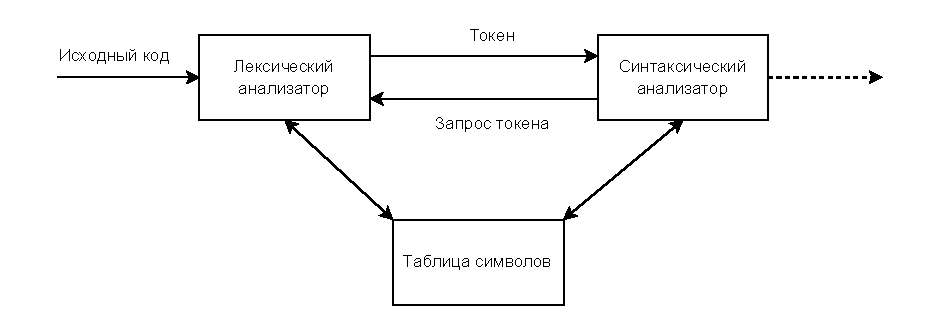
\includegraphics[width=0.9\textwidth]{structures/lexical_analyzer/la_sa_struct.pdf}
	\caption{Схема взаимодействия лексического и синтаксического анализаторов}
	\label{f:la_sa_struct}
\end{figure}

При запросе нового токена лексический анализатор считывает входной поток символов до точной идентификации следующего токена.

Процесс распознавания токенов из входного потока символов языка можно показать с помощью диаграмм переходов состояний.

На рисунке~\ref{f:dps_eq_assign} показана диаграмма для определения токенов «=» и «==».

\begin{figure}[ht]
	\centering
	\vspace{\toppaddingoffigure}
	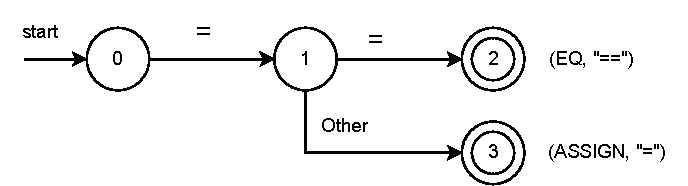
\includegraphics[width=0.9\textwidth]{structures/lexical_analyzer/dps_eq_assign.pdf}
	\caption{Диаграмма переходов для определения «=» и «==»}
	\label{f:dps_eq_assign}
\end{figure}

Работа начинается с состояния 0, в котором считывается следующий символ из входного потока.
Если полученный символ «=», то по дуге, помеченной «=» выполняется переход в состояние 1.
В состоянии 1 выполняется считывание следующего символа.
Если этот символ «=», выполняется переход в состояние 2 – заключительное состояние,
в котором найден токен «EQ», в том случае, если был получен символ отличный от «=»,
происходит переход по дуге «other» в состояние 3 с токеном «ASSIGN».

Диаграмма для распознавания целого числа представлена на рисунке~\ref{f:dps_int}.

\begin{figure}[ht]
	\centering
	\vspace{\toppaddingoffigure}
	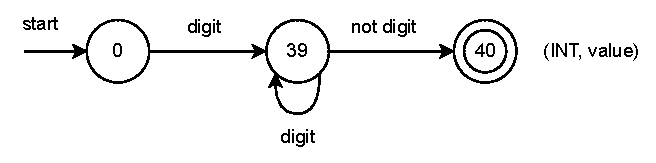
\includegraphics[width=0.9\textwidth]{structures/lexical_analyzer/dps_int.pdf}
	\caption{Диаграмма переходов для определения целого числа}
	\label{f:dps_int}
\end{figure}

При получении в начальном состоянии цифры, выполняется переход в состояние 39, в котором автомат находится до тех пор,
пока не получит на вход символ, отличный от цифры, при получении такого символа выполняется переход в конечное состояние 40.
По мере определения очередной цифры, она заносится в буфер.
В состоянии 40 возвращается токен INT и значение числа из буфера.

Считывание ключевых слов и идентификаторов показано с помощью диаграммы передов на рисунке~\ref{f:dps_ident_kw}.

Из начального состояния происходит переход в состояние 35, если была получена буква.
По аналогии с состоянием 39 выполняется циклическое считывание букв с занесением в буфер.
Если была получена не буква, выполняется переход в состояние 36, в котором проверяется принадлежность считанной строки к списку ключевых слов.
В случае, если считанная строка является ключевым словом, автомат переходит в завершающее состояние 37 в котором указывается тип токена для полученного ключевого слова и значение.
Если в состоянии 36 проверка показала, что строка на является ключевым словом, то выполняется переход в состояние 38 – определен идентификатор.

\begin{figure}[ht]
	\centering
	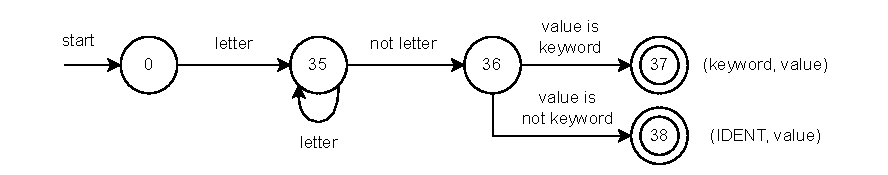
\includegraphics[width=0.9\textwidth]{structures/lexical_analyzer/dps_ident_kw.pdf}
	\caption{Диаграмма переходов для определения идентификаторов и ключевых слов}
	\label{f:dps_ident_kw}
\end{figure}

Полная диаграмма переходов состояний представлена на рисунке~\ref{f:full_dps}

Процесс распознавания токена начинается с начального состояния 0.
В зависимости от полученного символа выполняется переход в конкретное состояние.
Однако, если в начальном состоянии был получен символ, для которого нет дуги,
по которой он бы мог перейти в определенное для него состояние, выполняется переход по дуге «other» в состояние 42 с определением токена ILLEGAL.
После определения очередного токена в конечном состоянии, автомат начинает работу заново с начального состояния.
Считывание входного потока символов прекращается при поступлении нулевого символа (null character) с определением токена EOF.
Вместе с токеном, лексический анализатор возвращает его позицию в входном коде.

% В данном разделе была выполнена разработка структурных решений и алгоритмов функционирования лексического анализатора предметно-ориентированного языка.

\clearpage

\begin{figure}[h!]
	\centering
	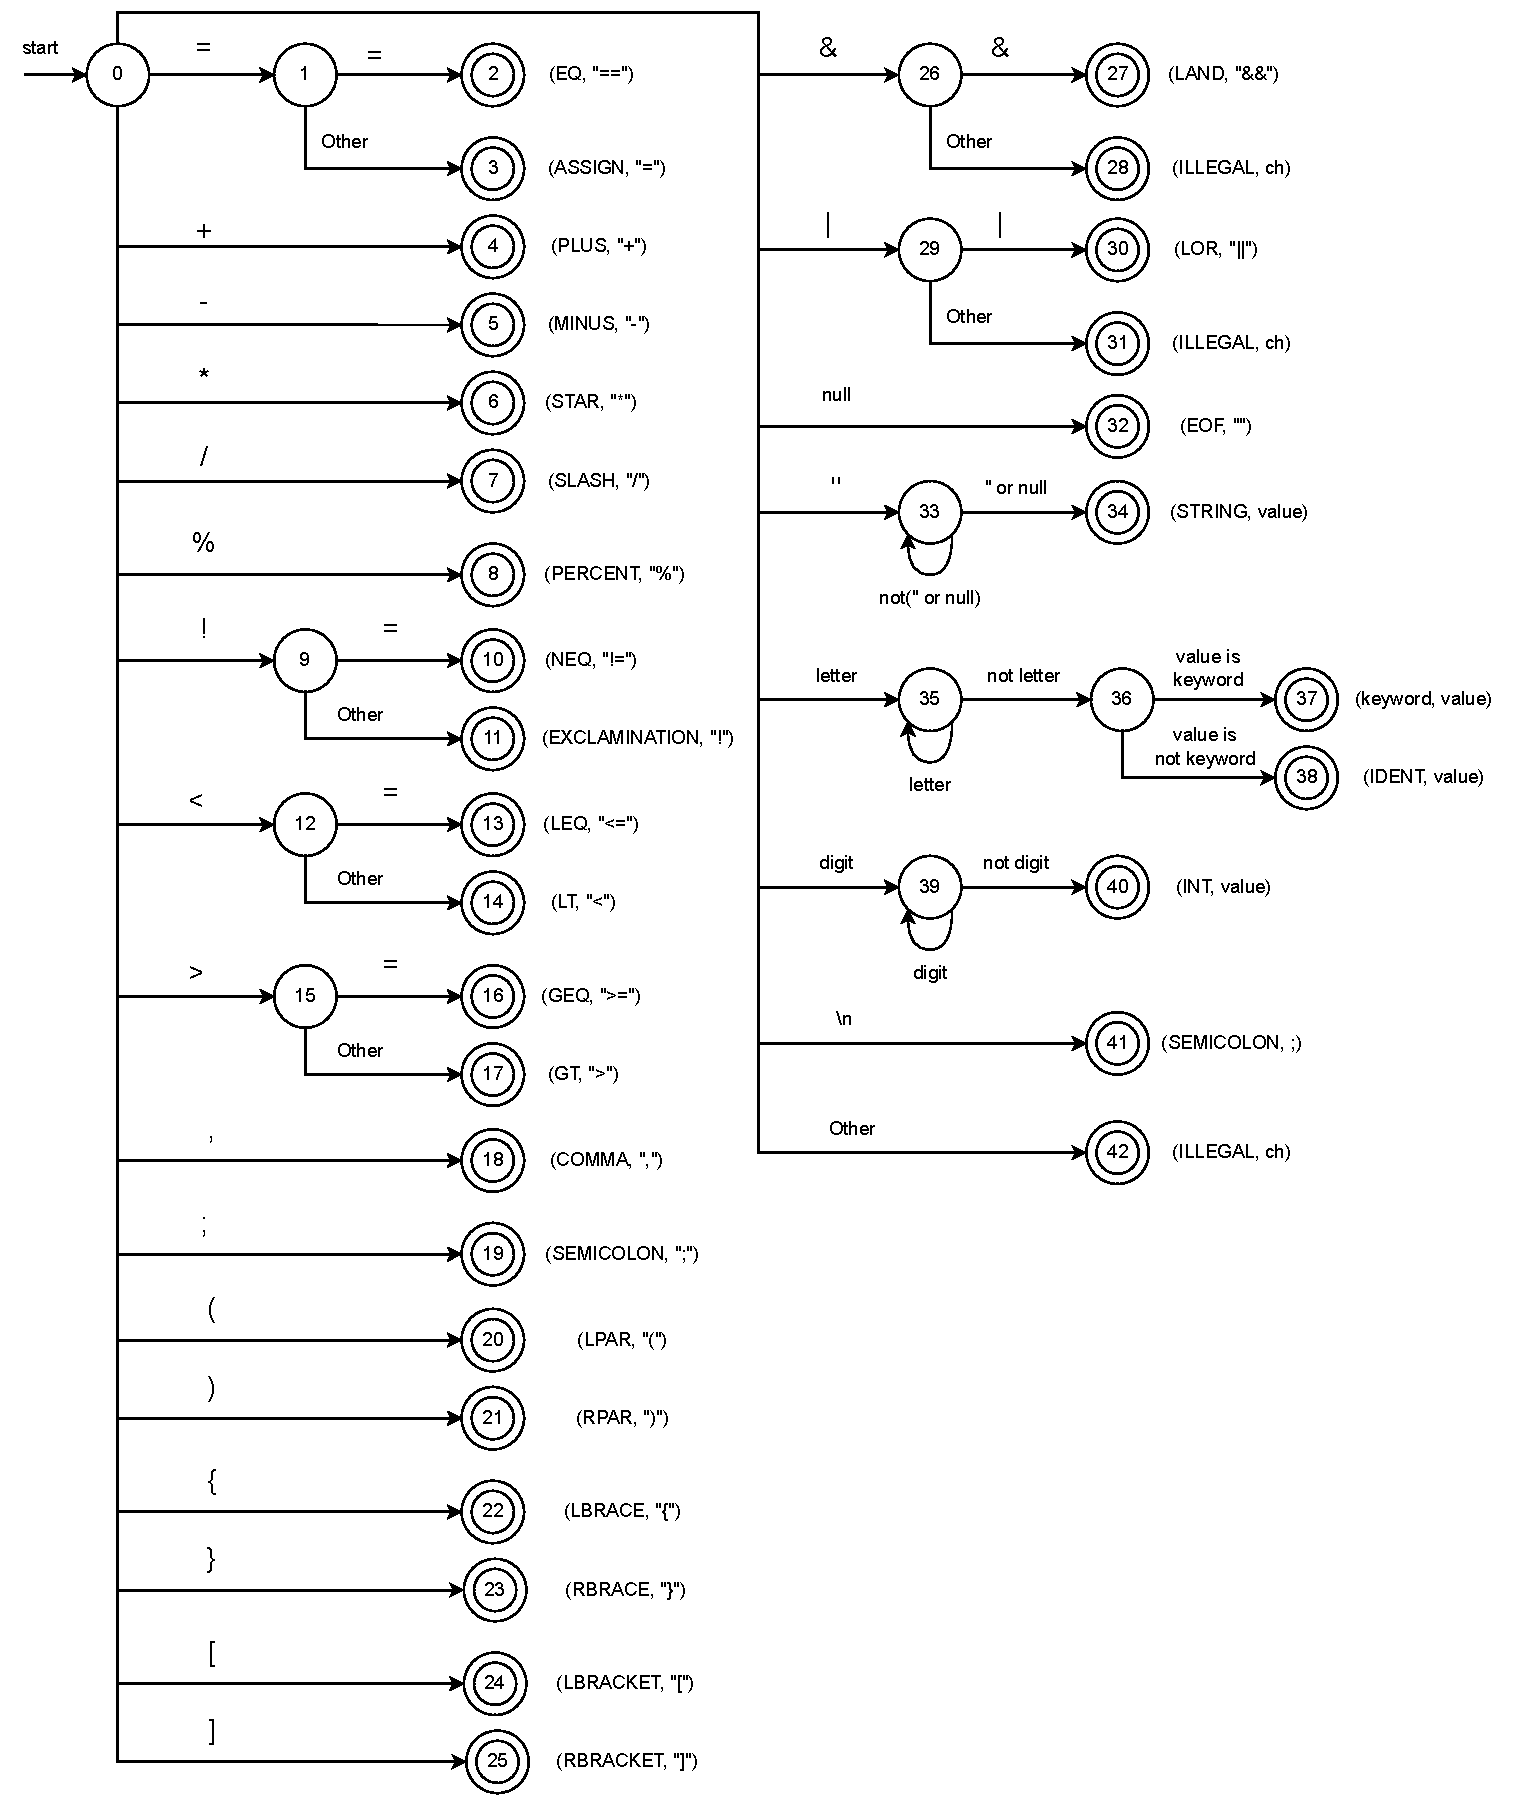
\includegraphics[width=1.0\textwidth]{structures/lexical_analyzer/full_dps.pdf}
	\caption{Полная диаграмма переходов состояний}
	\label{f:full_dps}
\end{figure}

\clearpage